\documentclass[11pt,a4paper]{article}

% Study 2 on Qwen3-32B: own starting value vs given starting value (29 October 2026).
% Figures: study2_figures.pdf, one figure per page, made by latex/study2_qwen3/figures.py
% from the data in the repository (data/pilot_v2/raw/qwen3-32b/study2/).

\usepackage[utf8]{inputenc}
\usepackage[T1]{fontenc}
\usepackage{lmodern}
\usepackage[margin=2.5cm]{geometry}
\usepackage{microtype}
\usepackage{amsmath,amssymb}
\usepackage{booktabs}
\usepackage{tabularx}
\usepackage{longtable}
\usepackage{array}
\usepackage{enumitem}
\usepackage{graphicx}
\usepackage[table]{xcolor}
\usepackage{textcomp}
\usepackage[most]{tcolorbox}
\usepackage[section]{placeins}
\usepackage[colorlinks=true,linkcolor=blue!50!black,urlcolor=blue!50!black]{hyperref}

\setlist{itemsep=2pt,topsep=4pt}
\setlength{\parskip}{3pt}
\newcolumntype{L}{>{\raggedright\arraybackslash}X}
\newcolumntype{R}{>{\raggedleft\arraybackslash}p{1.9cm}}

% one figure per page of this PDF
\newcommand{\fig}[2][\textwidth]{\includegraphics[page=#2,width=#1]{study2_figures.pdf}}

\definecolor{boxblue}{HTML}{EEF3FB}
\definecolor{boxline}{HTML}{2A78D6}
\definecolor{trgrey}{HTML}{F4F4F1}
\definecolor{trline}{HTML}{898781}
\definecolor{upcol}{HTML}{1BAF7A}
\definecolor{downcol}{HTML}{EB6834}

% a key message
\newtcolorbox{keybox}[1][]{breakable, colback=boxblue, colframe=boxline, boxrule=0pt, leftrule=3pt,
  arc=0pt, left=8pt, right=8pt, top=4pt, bottom=4pt, fonttitle=\bfseries, coltitle=black,
  title={#1}, attach title to upper={\ }, before skip=8pt, after skip=8pt}
% literal model text
\newtcolorbox{transcript}[1][]{breakable, colback=trgrey, colframe=trline, boxrule=0pt, leftrule=2pt,
  arc=0pt, left=8pt, right=8pt, top=4pt, bottom=4pt, fontupper=\small, fonttitle=\small\bfseries,
  coltitle=black, title={#1}, attach title to upper={\par\smallskip}, before skip=8pt, after skip=8pt}
\newcommand{\who}[1]{\par\smallskip\noindent\textsf{\textbf{\footnotesize\MakeUppercase{#1}}}\quad}
\newcommand{\cut}{\textup{[\dots]}}

\title{\textbf{Study 2 on Qwen3-32B}\\[4pt]
\large Does thinking help the model move away from its \emph{own} starting value more than from a \emph{given} one?\\[2pt]
\normalsize Project: \emph{Adjusting or Retrieving? Testing the Mechanisms of Anchoring in Large Language Models}}
\author{Hannan Seyfi\\[6pt]
\normalsize Supervisors: Dr.\ Shiva Kamkar and Dr.\ Babak Majidi\\
\normalsize Khatam University}
\date{29 October 2026}

\begin{document}
\maketitle

\begin{keybox}[The short version.]
\begin{itemize}[leftmargin=1.2em]
  \item We asked Qwen3-32B 10 questions, 1,800 times in total. Each question has a natural starting value: one Earth year (365 days) for an asteroid's orbit, or the previous film or Games for a 2026 event. In one version the model has to think of that value \textbf{itself}; in the other we \textbf{give} it (``Is it higher or lower than 365 days?'').
  \item \textbf{A given starting value pulls harder than the model's own.} Across the questions, answers moved about 0.1 to 0.4 less far away from it (on a scale where 0 = stayed at the start and 1 = reached the truth), at every thinking level (Figure~\ref{fig:main}).
  \item \textbf{Thinking helped in both versions.} With no extra sentence, thinking moved answers further from the start in both. It helped the model's own starting value a bit more (+0.44 against +0.28), but only in 5 or 6 of the 9 questions. So the strong prediction, \emph{``thinking helps only with the model's own starting value''}, is \textbf{not supported}. The weak version (``helps more'') is a trend, not a clear result.
  \item \textbf{The ``accuracy matters'' sentence behaved as in humans.} With thinking off, it helped the model's own starting value more than the given one in \textbf{all 9 questions}. ``Consider why it might be different'' helped both equally, which is also what human studies found. But these sentences made the model reason out loud in its answer (3 times longer), so ``no thinking'' was no longer really no thinking.
  \item \textbf{The thinking limit matters.} Short thinking (max 512 tokens) was stopped at the limit in 98\% of answers, often in the middle of a calculation. On the asteroid questions, short thinking was \emph{no better} than no thinking. ``Short'' really means ``interrupted''.
\end{itemize}
\end{keybox}

\section{What Study 2 asks}

When people estimate something, they often start from a number that comes to mind and adjust from it, usually not far enough. Human studies found a surprising difference. If people think of the starting number \emph{themselves}, more effort helps them move further from it. If someone \emph{gives} them the number, more effort does not help much. The explanation is that a self-made starting value is known to be wrong, so people keep adjusting, while a given value makes the mind look for reasons it might be right.

Study 2 asks whether a language model shows the same difference, and whether its \emph{thinking} plays the role of human effort. The prediction was: \textbf{thinking, and sentences asking for care, help the model move away from its own starting value, but not from a given one.}

\paragraph{An example.} ``How many Earth days does it take the asteroid 25143 Itokawa to orbit the Sun once?'' A natural first thought is one Earth year, 365 days. The true answer is 557 days.
\begin{itemize}
  \item \textbf{Own starting value:} we ask only the question. If the model starts from 365, it thought of it itself.
  \item \textbf{Given starting value:} we first ask ``Is it higher or lower than 365 days?'', then ask for the estimate.
\end{itemize}
The starting value is the same number in both versions. Only \emph{who brought it up} changes.

\subsection*{What we ran}

\begin{center}
\begin{tabular}{@{}ll@{}}
\toprule
Model & Qwen3-32B on DeepInfra (cost of this run: \$0.62) \\
Questions & 10: six asteroid orbits, two 2026 medal counts, two 2026 films \\
Starting value & own / given \\
Extra sentence & none / ``accuracy matters'' / ``consider why it might be different'' \\
Thinking & off / short (max 512 tokens) / long (max 2,048 tokens) \\
Repeats & 10 answers per question and condition \\
Total & $10 \times 2 \times 3 \times 3 \times 10 = 1{,}800$ answers \\
\bottomrule
\end{tabular}
\end{center}

The two extra sentences come from human studies. ``Accuracy matters here: take as much care as you need to make your estimate as close as possible to the true value'' is like paying people for accuracy. ``Before answering, consider reasons why the true value might be quite different from {[the first value that comes to mind / 365 days]}'' is the ``consider the opposite'' method.

\subsection*{The quick look in the notebook}

The notebook printed:
\begin{transcript}[]
\ttfamily\footnotesize study2  1800 answers | off: parsed 100\%, thinking 0 tok, cut off 0\% | low: parsed 100\%, thinking 511 tok, cut off 98\% | high: parsed 100\%, thinking 1572 tok, cut off 46\%
\end{transcript}
\emph{Parsed 100\%} means every answer had a number we could read (one answer out of 1,800 was an endless repeat of the film title, so the exact figure is 99.94\%). \emph{Thinking 511 tok} is the average length of the thinking. \emph{Cut off 98\%} means the thinking reached its limit and the model was told to stop and answer. Section~\ref{sec:cutoff} checks whether that matters. Baseline and Study 1 said ``no data yet'' only because this run did Study 2 alone.

\section{How we measure ``moving away''}

For each question and condition we take the \textbf{middle answer} (the median of the 10 answers), then ask how far it went from the starting value towards the true value:
\[
\text{moved} \;=\; \frac{\text{middle answer} - \text{starting value}}{\text{true value} - \text{starting value}}
\]
\textbf{0} means the answer stayed at the starting value; \textbf{1} means it reached the true value. Two examples:
\begin{itemize}
  \item Itokawa, own starting value, long thinking: middle answer 540. $(540-365)/(557-365) = 175/192 = 0.91$. Almost all the way.
  \item Bennu (true 436.65 days): the model answered 433 at \emph{every} level. $(433-365)/(436.65-365) = 0.95$. It simply knows this one, so there is nothing left to move. We leave Bennu out of the summaries (9 questions remain). In the screening it said 367 without thinking, so this changed between runs.
\end{itemize}
Values below 0 mean the answer went the wrong way; above 1 it overshot. To stop one odd answer from dominating, values are capped at $-0.5$ and $1.5$.

\section{Worked example 1: the Mario film}

``The film The Super Mario Galaxy Movie was released in cinemas in April 2026. How much did it earn at the worldwide box office?'' The previous film, \emph{The Super Mario Bros.\ Movie}, earned \$1,361 million. The new one earned \$1,013 million. The model was trained before 2026, so it cannot know this; it has to estimate.

\begin{figure}[ht]
\centering\fig{1}
\caption{Each dot is one answer (10 per group). The thick bar is the middle answer. Green = the model had to think of the previous film itself; purple = we asked ``higher or lower than 1,361?''.}
\label{fig:mario}
\end{figure}

This question shows the prediction exactly (Figure~\ref{fig:mario}). In \textbf{both} versions the model recalls the first film's \$1.36 billion. With its \textbf{own} starting value, thinking brings the middle answer down from 1,300 to 950, close to the true 1,013. With the \textbf{given} value, it stays at 1,450 and only drops to 1,350 with long thinking. Here are two long-thinking answers, word for word:

\begin{transcript}[Own starting value, long thinking (answer: 950)]
\who{thinking} \cut{} The most recent Mario movie was The Super Mario Bros. Movie in 2023, which was a huge hit. It made around \$1.36 billion worldwide. That's a solid benchmark. \cut{} perhaps it's safe to estimate around \$800 million to \$1.2 billion. \cut{} Maybe the Galaxy movie is a bit less, so maybe \$900 million. \cut{} Let's go with an estimate of \$950 million as a middle ground.
\end{transcript}

\begin{transcript}[Given starting value, long thinking (answer: 1,250)]
\who{thinking} \cut{} the Super Mario Bros. movie from 2023 \cut{} made around \$1.35 billion worldwide. That's just under \$1.361 billion. \cut{} So the comparison would be lower than \$1.361 billion. My estimate would be around \$1.3 billion, maybe a bit less. \cut{} If the first made \$1.35 billion, a sequel might make \$1.2 to \$1.3 billion. So I'll go with lower, and estimate \$1,250 million.
\who{answer} Comparison: lower \quad Estimate: 1250
\end{transcript}

The second answer is the textbook pattern of a given anchor: the model decides ``lower'', then goes only a little lower.

\section{Worked example 2: asteroid Itokawa}

\begin{figure}[ht]
\centering\fig{2}
\caption{Same layout as Figure~\ref{fig:mario}, for Itokawa (starting value 365 days, true value 557 days).}
\label{fig:itokawa}
\end{figure}

Here the result is different (Figure~\ref{fig:itokawa}). Without thinking and with short thinking, the middle answer stays near one year in both versions (369 and 367 with its own starting value; 396 and 406 with the given one). With long thinking \textbf{both} versions reach the truth: 540 and 528. The model works it out with Kepler's law (``semi-major axis about 1.3 AU, $P^2 = 1.3^3$, so about 1.48 years, about 540 days''), and that works whoever brought up the 365. So for Itokawa, thinking helped in both versions equally.

\section{The main result}

\begin{figure}[ht]
\centering\fig[0.75\textwidth]{3}
\caption{How far the middle answer moved from the starting value (0) towards the truth (1), as the middle of the 9 questions (Bennu left out). No extra sentence.}
\label{fig:main}
\end{figure}

Figure~\ref{fig:main} shows two things.
\begin{enumerate}
  \item \textbf{The given value always pulls harder.} The purple line is below the green one at every thinking level. Without thinking, answers with a given starting value did not move at all (0.00); with its own they moved a little (0.18).
  \item \textbf{Thinking helps in both versions.} Own starting value: $0.18 \to 0.53 \to 0.62$ (+0.44). Given: $0.00 \to 0.18 \to 0.28$ (+0.28). Thinking helped the own version a bit more, but the given version clearly improved too. The prediction said it would not.
\end{enumerate}

Is the ``bit more'' reliable? Counted question by question, thinking helped the own version more than the given version in \textbf{6 of 9} questions with short thinking and \textbf{5 of 9} with long thinking. That is close to a coin flip. Figure~\ref{fig:items} shows each question.

\begin{figure}[ht]
\centering\fig{4}
\caption{Every question on its own, no extra sentence. Dashed line = starting value, dotted line = truth.}
\label{fig:items}
\end{figure}

\paragraph{One warning about the 2026 questions.} The ``own starting value'' only works if the model actually thinks of it. We checked how often the model's own-version replies mention the previous value:

\begin{center}
\small
\begin{tabular}{@{}lrrr@{}}
\toprule
Question (own starting value) & no thinking & short & long \\
\midrule
Asteroids (365 days), range over 6 questions & 20--70\% & 57--80\% & 100\% \\
Mario Galaxy (previous film \$1,361 m) & 80\% & 60\% & 90\% \\
Japan, Asian Games medals (previous 188) & 0\% & 0\% & 0\% \\
Canada, Commonwealth Games medals (previous 92) & 3\% & 0\% & 0\% \\
Now You See Me 3 (previous film \$334.9 m) & 0\% & 7\% & 10\% \\
\bottomrule
\end{tabular}
\end{center}

For three of the four 2026 questions the model almost never recalls the previous value, so in the ``own'' version it has no starting value at all. For those questions the green line is really ``no starting value'', and the gap to the purple line is just ordinary anchoring. The asteroid questions and the Mario film are the fair test. On those six questions there is still no clear difference: with short thinking the own version moved more (0.18 to 0.49, against $-0.01$ to 0.05 for given), but with long thinking the given version caught up (own 0.29, given 0.23). Thinking helped the own version more in 4 of 6 questions with short thinking and 3 of 6 with long thinking.

\section{The extra sentences}

\begin{figure}[ht]
\centering\fig{5}
\caption{The same measure for each extra sentence (middle of 9 questions).}
\label{fig:instr}
\end{figure}

\begin{figure}[ht]
\centering\fig{6}
\caption{Thinking off only. A: how far answers moved. B: average length of the visible answer.}
\label{fig:off}
\end{figure}

With thinking off, the sentences had a large effect (Figure~\ref{fig:off}A):
\begin{itemize}
  \item \textbf{``Accuracy matters''} moved answers further with the model's own starting value (+0.20, middle of 9 questions) than with a given one (+0.06). It helped the own version more in \textbf{all 9 questions}. This matches human studies: paying people for accuracy helps only with self-made starting values (Epley and Gilovich, 2005).
  \item \textbf{``Consider why it might be different''} helped both versions about equally (+0.25 own, +0.28 given). This also matches humans: ``consider the opposite'' is the one method known to reduce anchoring on \emph{given} values (Mussweiler, Strack and Pfeiffer, 2000).
\end{itemize}

But Figure~\ref{fig:off}B shows a catch. With either sentence, the visible answer became about \textbf{three times longer} (about 330 tokens instead of about 110). The model did its reasoning out loud in the answer. For example, for Itokawa with ``accuracy matters'' and no thinking it wrote: ``According to NASA's JPL Small-Body Database, the orbital period of 25143 Itokawa is 1.622013 years \cut{} $1.622013 \times 365.25 = 592.74$ days'' (true value 557). So ``no thinking'' plus a sentence is really ``thinking in the answer, with no limit''. Once real thinking is on (Figure~\ref{fig:instr}, middle and right), the sentences add little, and the own/given difference is about the same as without a sentence.

\section{Does the thinking limit matter?}
\label{sec:cutoff}

\begin{figure}[ht]
\centering\fig{7}
\caption{A: thinking length of every answer. Tall bars at 512 and 2,048 are answers stopped at the limit. B: asteroid questions only (Bennu left out), own and given together; one line per extra sentence.}
\label{fig:cutoff}
\end{figure}

Yes. Figure~\ref{fig:cutoff}A shows that almost every short-thinking answer was stopped at 512 tokens. The model then has to answer straight away, with whatever it had in mind. Sometimes that is the middle of a calculation, and it falls back to the starting value:

\begin{transcript}[Itokawa, own starting value, short thinking: stopped at 512 tokens (answer: 367)]
\who{thinking} \cut{} maybe its semi-major axis is around 1.3 AU. \cut{} If Itokawa's semi-major axis is similar, say around 1.3 AU, then using Kepler's law, P squared would be (1.3)\^{}3. Let me calculate that. 1.3 cubed is 1.3 * 1.3 = 1.69, then 1.69 * 1.3 $\approx$ 2.197. So P squared is approximately 2.197, so P is the square root of
\who{answer} Estimate: 367
\end{transcript}

The model was one step from about 540 days, but the limit stopped it and it answered 367. This is ``insufficient adjustment'' produced by the limit, not by the model.

Figure~\ref{fig:cutoff}B shows the effect on the asteroid questions. Short thinking barely beat no thinking (0.09 to 0.17 with no sentence), and with ``accuracy matters'' it was much \emph{worse} (0.59 to 0.17): without thinking the model could reason freely in the answer, while short thinking cut the reasoning off at 512 tokens and then gave a one-line answer. Even long thinking hit its 2,048 limit in 68--83\% of the asteroid answers. Within the same condition, long-thinking answers that hit the limit were further from the truth than those that finished (middle error 0.44 against 0.30 on a log scale), though only in 22 of 39 conditions, so this is a weak sign.

\textbf{What this means for the study.} The own/given comparison is still fair, because both versions get the same limit. But the thinking levels do not mean what we wanted: ``short'' is ``interrupted'', not ``short but finished''. Any claim about \emph{how much} thinking helps needs limits the model rarely hits.

\section{Honest notes}
\begin{itemize}
  \item This is a pilot: one model, 10 questions (9 usable), 10 answers per condition. Differences of 0.1 to 0.2 in Figures~\ref{fig:main}--\ref{fig:instr} could change with more questions.
  \item The summaries are medians over questions. A different summary (for example the mean) gives the same direction but different sizes.
  \item For the 2026 questions the model cannot know the truth, so ``moving towards the truth'' partly means ``guessing the right direction''. The asteroid questions do not have this problem.
  \item Several question-selection rules were set after seeing screening data (see CHANGELOG.md). Bennu passed the screening but was fully known in this run.
\end{itemize}

\section{What we learned, and what next}

\begin{enumerate}
  \item \textbf{Given starting values pull harder than the model's own,} at every thinking level. This is a clean result.
  \item \textbf{Thinking does not only help with the model's own starting value.} It helps with given ones too. The main prediction, in its strong form, did not hold on this model.
  \item \textbf{``Accuracy matters'' helps own starting values more (9 of 9 questions), ``consider the opposite'' helps both,} as in humans. But this happened through reasoning written in the answer, which we did not control.
  \item \textbf{The 512-token limit interrupts the thinking} and makes the short level hard to interpret.
\end{enumerate}

\paragraph{Suggested next run (cheap, about \$1 on DeepInfra):}
\begin{itemize}
  \item \textbf{Raise the limits} to 1,024 (short) and 4,096 (long), or add a level where the model thinks until it stops by itself, so that most answers finish.
  \item \textbf{Make ``no thinking'' truly short:} ask for the number only (``Reply with only the Estimate line''), so the extra sentences cannot turn into written-out reasoning.
  \item \textbf{Keep only questions where the model really thinks of the starting value} (asteroids, Mario-like films) and add more of them, so we have more than 6 fair questions.
  \item Run the same on a smaller model (Qwen3-14B or 8B) to see whether the own/given gap grows when the model knows less.
\end{itemize}

\end{document}
